\documentclass{standalone}
\usepackage{tikz}
\usetikzlibrary{patterns, positioning}


\begin{document}
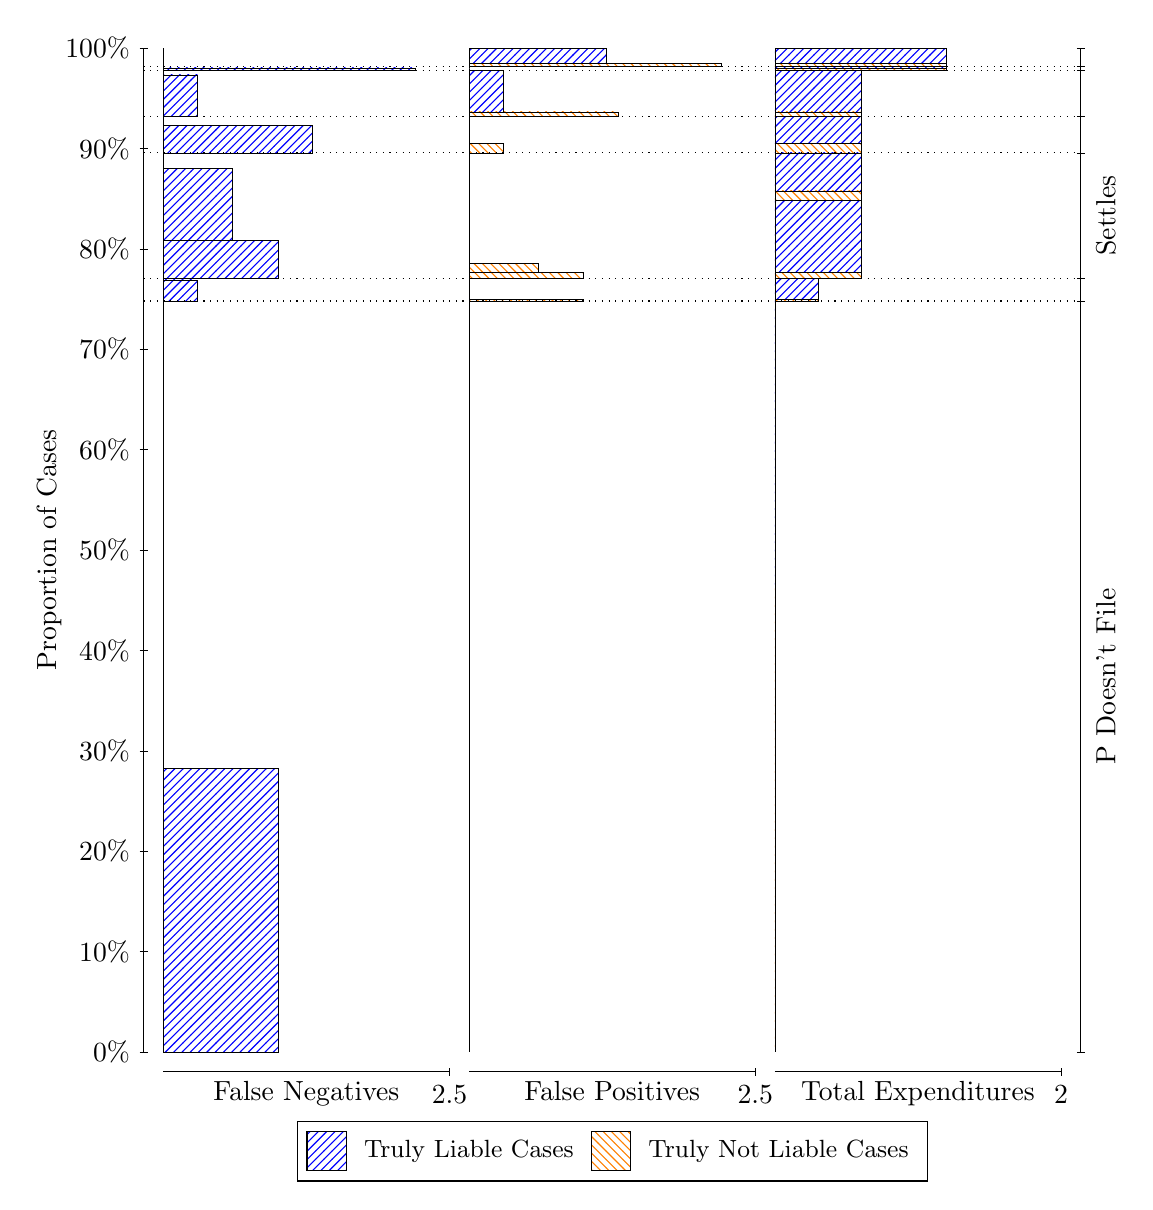
\begin{tikzpicture}
\draw[black, very thin] (1.5,1.75) -- (1.5,14.5);
\node[rotate=90, text=black, anchor=center] at (0.3, 8.125) {Proportion of Cases};
\draw[black, very thin] (1.45,1.75) -- (1.55,1.75);
\node[text=black, anchor=east] at (1.45, 1.75) {0\%};
\draw[black, very thin] (1.45,3.025) -- (1.55,3.025);
\node[text=black, anchor=east] at (1.45, 3.025) {10\%};
\draw[black, very thin] (1.45,4.3) -- (1.55,4.3);
\node[text=black, anchor=east] at (1.45, 4.3) {20\%};
\draw[black, very thin] (1.45,5.575) -- (1.55,5.575);
\node[text=black, anchor=east] at (1.45, 5.575) {30\%};
\draw[black, very thin] (1.45,6.85) -- (1.55,6.85);
\node[text=black, anchor=east] at (1.45, 6.85) {40\%};
\draw[black, very thin] (1.45,8.125) -- (1.55,8.125);
\node[text=black, anchor=east] at (1.45, 8.125) {50\%};
\draw[black, very thin] (1.45,9.4) -- (1.55,9.4);
\node[text=black, anchor=east] at (1.45, 9.4) {60\%};
\draw[black, very thin] (1.45,10.675) -- (1.55,10.675);
\node[text=black, anchor=east] at (1.45, 10.675) {70\%};
\draw[black, very thin] (1.45,11.95) -- (1.55,11.95);
\node[text=black, anchor=east] at (1.45, 11.95) {80\%};
\draw[black, very thin] (1.45,13.225) -- (1.55,13.225);
\node[text=black, anchor=east] at (1.45, 13.225) {90\%};
\draw[black, very thin] (1.45,14.5) -- (1.55,14.5);
\node[text=black, anchor=east] at (1.45, 14.5) {100\%};

\draw[black, very thin] (13.4,1.75) -- (13.4,14.5);
\draw[black, very thin] (13.35,1.75) -- (13.45,1.75);
\node[anchor=west] at (13.35, 1.75) {};
\draw[black, very thin] (13.35,11.287) -- (13.45,11.287);
\node[anchor=west] at (13.35, 11.287) {};
\draw[black, very thin] (13.35,11.578) -- (13.45,11.578);
\node[anchor=west] at (13.35, 11.578) {};
\draw[black, very thin] (13.35,13.168) -- (13.45,13.168);
\node[anchor=west] at (13.35, 13.168) {};
\draw[black, very thin] (13.35,13.63) -- (13.45,13.63);
\node[anchor=west] at (13.35, 13.63) {};
\draw[black, very thin] (13.35,14.218) -- (13.45,14.218);
\node[anchor=west] at (13.35, 14.218) {};
\draw[black, very thin] (13.35,14.269) -- (13.45,14.269);
\node[anchor=west] at (13.35, 14.269) {};
\draw[black, very thin] (13.35,14.5) -- (13.45,14.5);
\node[anchor=west] at (13.35, 14.5) {};

\draw[black, very thin, pattern color=blue, pattern=north east lines] (1.75,1.75) rectangle (3.2033,5.3552);
\draw[black, very thin, pattern color=orange, pattern=north west lines] (1.75,5.3552) rectangle (1.75,11.287);
\draw[black, very thin, pattern color=blue, pattern=north east lines] (1.75,11.287) rectangle (2.186,11.555);
\draw[black, very thin, pattern color=orange, pattern=north west lines] (1.75,11.555) rectangle (1.75,11.578);
\draw[black, very thin, pattern color=blue, pattern=north east lines] (1.75,11.578) rectangle (3.2033,12.06);
\draw[black, very thin, pattern color=blue, pattern=north east lines] (1.75,12.06) rectangle (2.622,12.976);
\draw[black, very thin, pattern color=orange, pattern=north west lines] (1.75,12.976) rectangle (1.75,13.168);
\draw[black, very thin, pattern color=blue, pattern=north east lines] (1.75,13.168) rectangle (3.6393,13.513);
\draw[black, very thin, pattern color=orange, pattern=north west lines] (1.75,13.513) rectangle (1.75,13.63);
\draw[black, very thin, pattern color=blue, pattern=north east lines] (1.75,13.63) rectangle (2.186,14.158);
\draw[black, very thin, pattern color=orange, pattern=north west lines] (1.75,14.158) rectangle (1.75,14.218);
\draw[black, very thin, pattern color=blue, pattern=north east lines] (1.75,14.218) rectangle (4.9473,14.249);
\draw[black, very thin, pattern color=orange, pattern=north west lines] (1.75,14.249) rectangle (1.75,14.269);
\draw[black, very thin, pattern color=orange, pattern=north west lines] (1.75,14.269) rectangle (1.75,14.3);
\draw[black, very thin, pattern color=blue, pattern=north east lines] (1.75,14.3) rectangle (1.75,14.5);
\draw[black, very thin, pattern color=orange, pattern=north west lines] (5.6333,1.75) rectangle (5.6333,7.6814);
\draw[black, very thin, pattern color=blue, pattern=north east lines] (5.6333,7.6814) rectangle (5.6333,11.287);
\draw[black, very thin, pattern color=orange, pattern=north west lines] (5.6333,11.287) rectangle (7.0867,11.309);
\draw[black, very thin, pattern color=blue, pattern=north east lines] (5.6333,11.309) rectangle (5.6333,11.578);
\draw[black, very thin, pattern color=orange, pattern=north west lines] (5.6333,11.578) rectangle (7.0867,11.65);
\draw[black, very thin, pattern color=orange, pattern=north west lines] (5.6333,11.65) rectangle (6.5053,11.769);
\draw[black, very thin, pattern color=blue, pattern=north east lines] (5.6333,11.769) rectangle (5.6333,13.168);
\draw[black, very thin, pattern color=orange, pattern=north west lines] (5.6333,13.168) rectangle (6.0693,13.285);
\draw[black, very thin, pattern color=blue, pattern=north east lines] (5.6333,13.285) rectangle (5.6333,13.63);
\draw[black, very thin, pattern color=orange, pattern=north west lines] (5.6333,13.63) rectangle (7.5227,13.69);
\draw[black, very thin, pattern color=blue, pattern=north east lines] (5.6333,13.69) rectangle (6.0693,14.218);
\draw[black, very thin, pattern color=orange, pattern=north west lines] (5.6333,14.218) rectangle (5.6333,14.238);
\draw[black, very thin, pattern color=blue, pattern=north east lines] (5.6333,14.238) rectangle (5.6333,14.269);
\draw[black, very thin, pattern color=orange, pattern=north west lines] (5.6333,14.269) rectangle (8.8307,14.3);
\draw[black, very thin, pattern color=blue, pattern=north east lines] (5.6333,14.3) rectangle (7.3773,14.5);
\draw[black, very thin, pattern color=orange, pattern=north west lines] (9.5167,1.75) rectangle (9.5167,7.6814);
\draw[black, very thin, pattern color=blue, pattern=north east lines] (9.5167,7.6814) rectangle (9.5167,11.287);
\draw[black, very thin, pattern color=orange, pattern=north west lines] (9.5167,11.287) rectangle (10.062,11.309);
\draw[black, very thin, pattern color=blue, pattern=north east lines] (9.5167,11.309) rectangle (10.062,11.578);
\draw[black, very thin, pattern color=orange, pattern=north west lines] (9.5167,11.578) rectangle (10.607,11.65);
\draw[black, very thin, pattern color=blue, pattern=north east lines] (9.5167,11.65) rectangle (10.607,12.565);
\draw[black, very thin, pattern color=orange, pattern=north west lines] (9.5167,12.565) rectangle (10.607,12.685);
\draw[black, very thin, pattern color=blue, pattern=north east lines] (9.5167,12.685) rectangle (10.607,13.168);
\draw[black, very thin, pattern color=orange, pattern=north west lines] (9.5167,13.168) rectangle (10.607,13.285);
\draw[black, very thin, pattern color=blue, pattern=north east lines] (9.5167,13.285) rectangle (10.607,13.63);
\draw[black, very thin, pattern color=orange, pattern=north west lines] (9.5167,13.63) rectangle (10.607,13.69);
\draw[black, very thin, pattern color=blue, pattern=north east lines] (9.5167,13.69) rectangle (10.607,14.218);
\draw[black, very thin, pattern color=orange, pattern=north west lines] (9.5167,14.218) rectangle (11.697,14.238);
\draw[black, very thin, pattern color=blue, pattern=north east lines] (9.5167,14.238) rectangle (11.697,14.269);
\draw[black, very thin, pattern color=orange, pattern=north west lines] (9.5167,14.269) rectangle (11.697,14.3);
\draw[black, very thin, pattern color=blue, pattern=north east lines] (9.5167,14.3) rectangle (11.697,14.5);
\draw[black, dotted] (1.5,11.287) -- (13.4,11.287);
\draw[black, dotted] (1.5,11.578) -- (13.4,11.578);
\draw[black, dotted] (1.5,13.168) -- (13.4,13.168);
\draw[black, dotted] (1.5,13.63) -- (13.4,13.63);
\draw[black, dotted] (1.5,14.218) -- (13.4,14.218);
\draw[black, dotted] (1.5,14.269) -- (13.4,14.269);
\draw[black, very thin] (1.75,1.5) -- (5.3833,1.5);
\node[text=black, anchor=north] at (3.5667, 1.5) {False Negatives};
\draw[black, very thin] (5.3833,1.45) -- (5.3833,1.55);
\node[text=black, anchor=north] at (5.3833, 1.45) {2.5};

\draw[black, very thin] (5.6333,1.5) -- (9.2667,1.5);
\node[text=black, anchor=north] at (7.45, 1.5) {False Positives};
\draw[black, very thin] (9.2667,1.45) -- (9.2667,1.55);
\node[text=black, anchor=north] at (9.2667, 1.45) {2.5};

\draw[black, very thin] (9.5167,1.5) -- (13.15,1.5);
\node[text=black, anchor=north] at (11.333, 1.5) {Total Expenditures};
\draw[black, very thin] (13.15,1.45) -- (13.15,1.55);
\node[text=black, anchor=north] at (13.15, 1.45) {2};

\node[text=black, centered, rotate=90] at (13.72, 6.5183) {P Doesn't File};

\node[text=black, centered, rotate=90] at (13.72, 12.373) {Settles};





\draw (7.449999999999999,1.5) node[draw=none] (baseCoordinate) {};
\begin{scope}[align=center]
        \matrix[scale=0.5, draw=black, below=0.5cm of baseCoordinate, nodes={draw}, column sep=0.1cm]{
            \node[rectangle, draw, minimum width=0.5cm, minimum height=0.5cm, pattern color=blue, pattern=north east lines] {}; &
            \node[draw=none, font=\small, text=black] (B) {Truly Liable Cases}; &
            \node[rectangle, draw, minimum width=0.5cm, minimum height=0.5cm, pattern color=orange, pattern=north west lines] {}; &
            \node[draw=none, font=\small, text=black] (B) {Truly Not Liable Cases}; \\
            };
\end{scope}

\end{tikzpicture}
\end{document}